\documentclass[border=5pt]{standalone}
\usepackage[utf8]{inputenc}
\usepackage{amsmath}
\usepackage{tikz}
\usetikzlibrary{positioning, fit, shapes}
\usetikzlibrary{chains}
\usetikzlibrary{calc}
\usetikzlibrary{decorations.pathmorphing}
\usetikzlibrary{shapes.multipart}
\usetikzlibrary{decorations,arrows}
\usetikzlibrary{decorations.pathmorphing}
\usepgflibrary{decorations.pathreplacing} 

\begin{document}

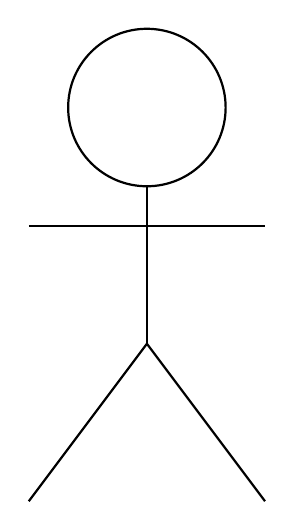
\begin{tikzpicture}[node distance=0cm, font=\sffamily]

% Head
\draw[thick] (0, 0) circle(1);

% Torso
\draw[thick] (0, -1) -- (0, -3);

% Arms
\draw[thick] (-1.5, -1.5) -- (1.5, -1.5);

% Legs
\draw[thick] (0, -3) -- (-1.5, -5); % Left
\draw[thick] (0, -3) -- (1.5, -5); % Right

\end{tikzpicture}

\end{document}
